\section{Processing}
\label{chap:processing}

\subsection{Epoching}
    We used the triggering signals from the behavioral box to select the intervals of interest. For each trial, we considered only the spikes that occurred 500 ms before the head-entry was detected -- when the infrared beam of the nosepoke was interrupted -- and those that occurred up to the withdrawal of the nosepoke. 
    
    \begin{figure}
        \centering
        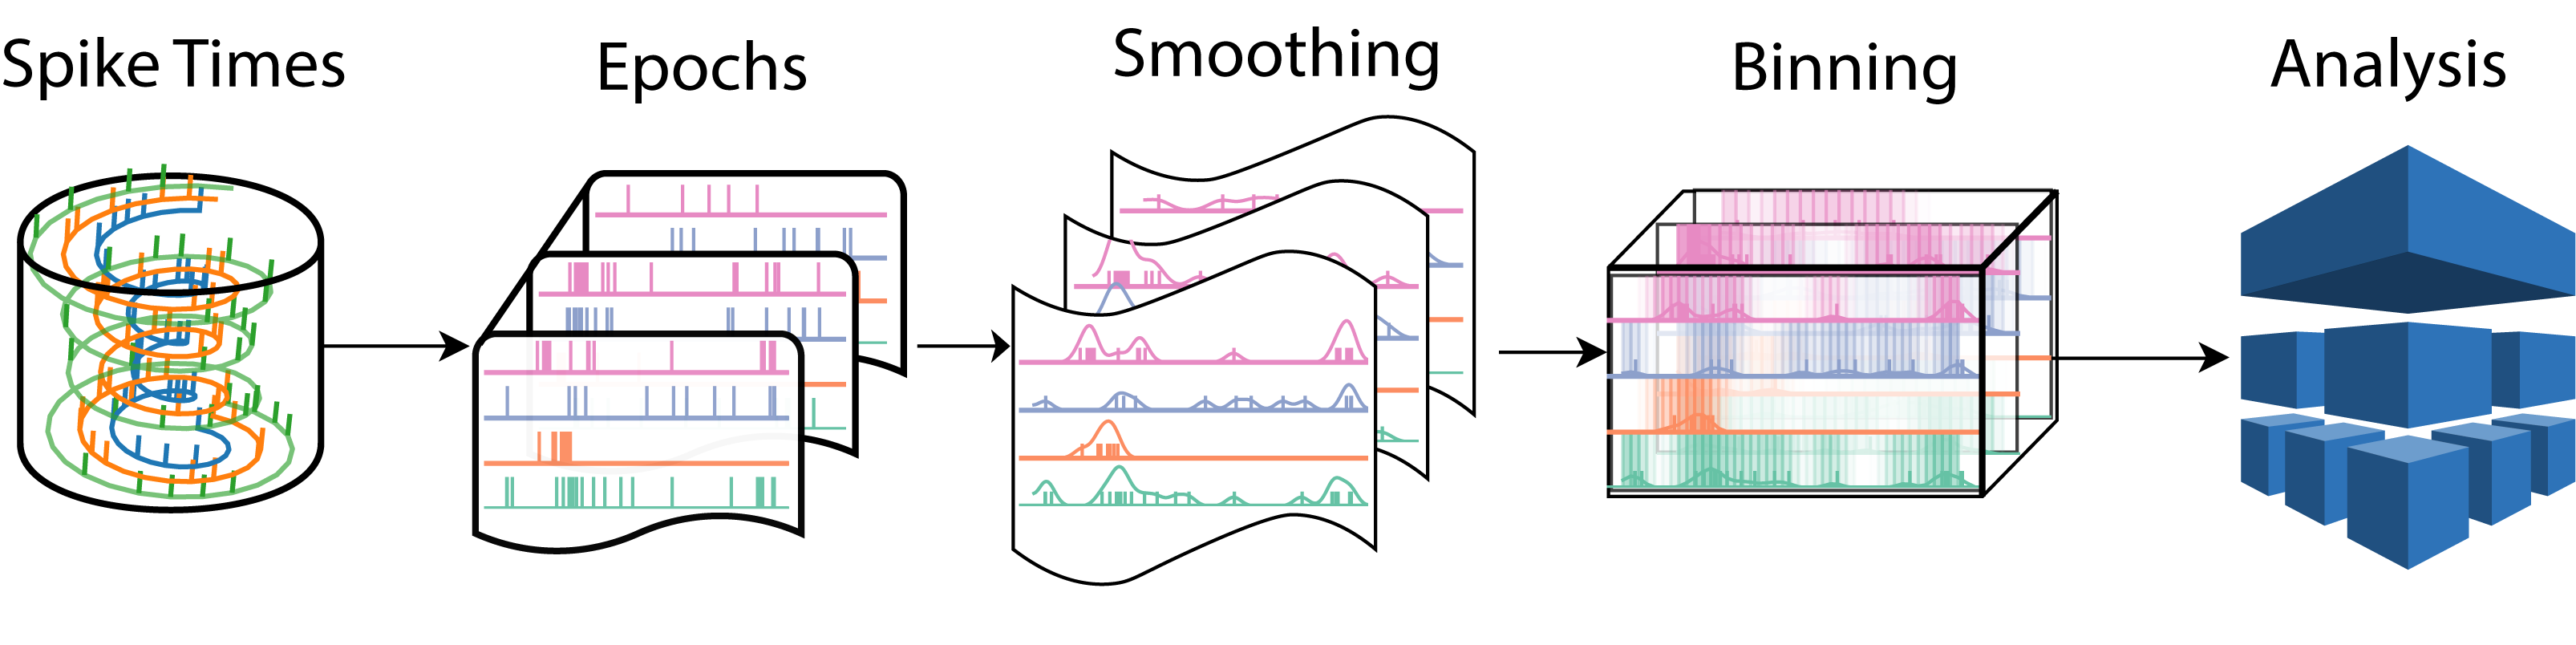
\includegraphics[width=\textwidth]{figures/Pipeline.png}
        \caption[Spike pre-processing steps]{Spike pre-processing steps: Spike times are epoched according to the nosepoke onsets, then smoothed to their estimated firing rate, and finally binned in equal-sized time bins, before being analyzed by machine learning. In the three intermediate steps we can see the activity of four neurons, in three different trials, through the pre-processing steps.}
        \label{fig:preproc}
    \end{figure} 
    
    % We divide spikes into their corresponding trials by using the events measured by our box. For each trial, we get all spikes that occurred between baseline (500ms before trial onset) and trial offset. This means it is possible to have the same spike in two trials, in cases when the intertrial interval is less than the baseline duration of 500ms, which was considered non-problematic.
    % \subsection{Firing rate estimation}
    % Before convolving we have to transform the time stamps into a boolean timeseries, for which we choose the precision of 1ms. Each neuron has then a time series of zeros and ones, with ones in times where the neuron was spiking.e

\subsection{Firing Rate estimation}
\label{subsec:fr_estimation}
    %We transformed the spike time-stamps into firing rates by convolving them with a gaussian \textit{kernel}, with standard deviation $\sigma = 100ms$ and symmetric padding, to avoid creating temporal information which would appear in the case of zero padding. After the convolution, we bin the spikes into windows of 100ms. For a given time bin we have a vector of activity, representing neurons' mean firing rate during those 100ms. Each dimension in this vector represents a different neuron.
    
    %For each trial, we analyze the activity from nosepoke onset until nosepoke removal. Over this interval, the activity from each neuron simultaneously recorded was transformed into firing rate by convolving with a gaussian and then averaging inside bins of 100ms. This procedure resulted in one population firing rate vector per 100 ms time bin, to a total of 15 vectors for 1.5s trials, 30 vectors for 3s trials, and so on. Only the first 15 bins were used for the analysis of bigger trials. 

    For each trial, we analyzed the spike activity from nosepoke onset until nosepoke removal. Within this interval, the activity from each neuron recorded was transformed into a firing rate. This conversion was conducted by convolving each spike with a gaussian \textit{kernel}, of standard deviation $\sigma = 100$~ms and symmetric padding, which avoids introducing artificial temporal information as it happens with zero padding (see Chapter \ref{chap:data_processing}).
    
    After the convolution, we calculate a histogram by counting spikes contained in windows (bins) of 100~ms. For a given time bin we have a vector of activity, representing the average firing rate of neurons during those 100ms. Each coordinate in this vector represents a different neuron. This procedure resulted in one population firing rate vector per 100 ms time bin, to a total of 15 vectors for 1.5s trials, 30 vectors for 3s trials, and so on. Only the first 15 bins were used for the analysis of trials longer than 1.5s.

    % We used three values for the standard deviation (20, 50 and 100), to assess the robustness of our analysis with respect to this parameter. To test the effects of different padding choices in estimating the firing rate, we compared the spike count (not smoothed) in 100ms bins with the firing rates measured using a gaussian kernel with standard deviation of 100ms, calculating the borders with either the default zero padding or a symmetric padding. At last we used the
    %, 50 and 20 ms. While the windows of 100 and 50 can be used for computationally expensive analysis, The window of 20ms is stored for visualization purposes.

\subsection{Disengagement exclusion}
    Inter trial interval, or ITI, is the time between two nosepokes. Specifically, it is the interval from when the animal exits the nosepoke until it enters again.
    The level of engagement was assessed using the inter trial interval of each animal. For such, we calculated the sum of ITIs occurring within a moving window of 5 trials. The first occurrence of a sum bigger than 5 minutes inside a window was defined as the disengagement point. All posterior trials to the disengagement were removed from further analysis.
    
\subsection{Correct trials}
    Unless otherwise specified, we selected as correct trials all rewarded trials (t > 1.5s) for our analysis, after the removal of trials without engagement. 
    
\subsection{Neuron pool}
    As typically done in the literature, we merged cells from all rats in most analysis. Correct trials were ordered and aligned for each group of animals, from the first trial of each animal to the last trial of the animal with the smallest session.
    
\subsection{Precaching}
    Because smoothing the data is computationally expensive, we saved smoothed firing rates of the all neurons from all rats to enable easier exploration and experimentation. The analyses were made by reading the smoothed data since it is computationally cheaper. 
    
